	 \section*{Apéndice A. Planos de manufactura}\label{sec:planos de manufactura}
  \addcontentsline{toc}{section}{Apéndice A. Planos de manufactura}
	\begin{figure}[h!]
	\centering
	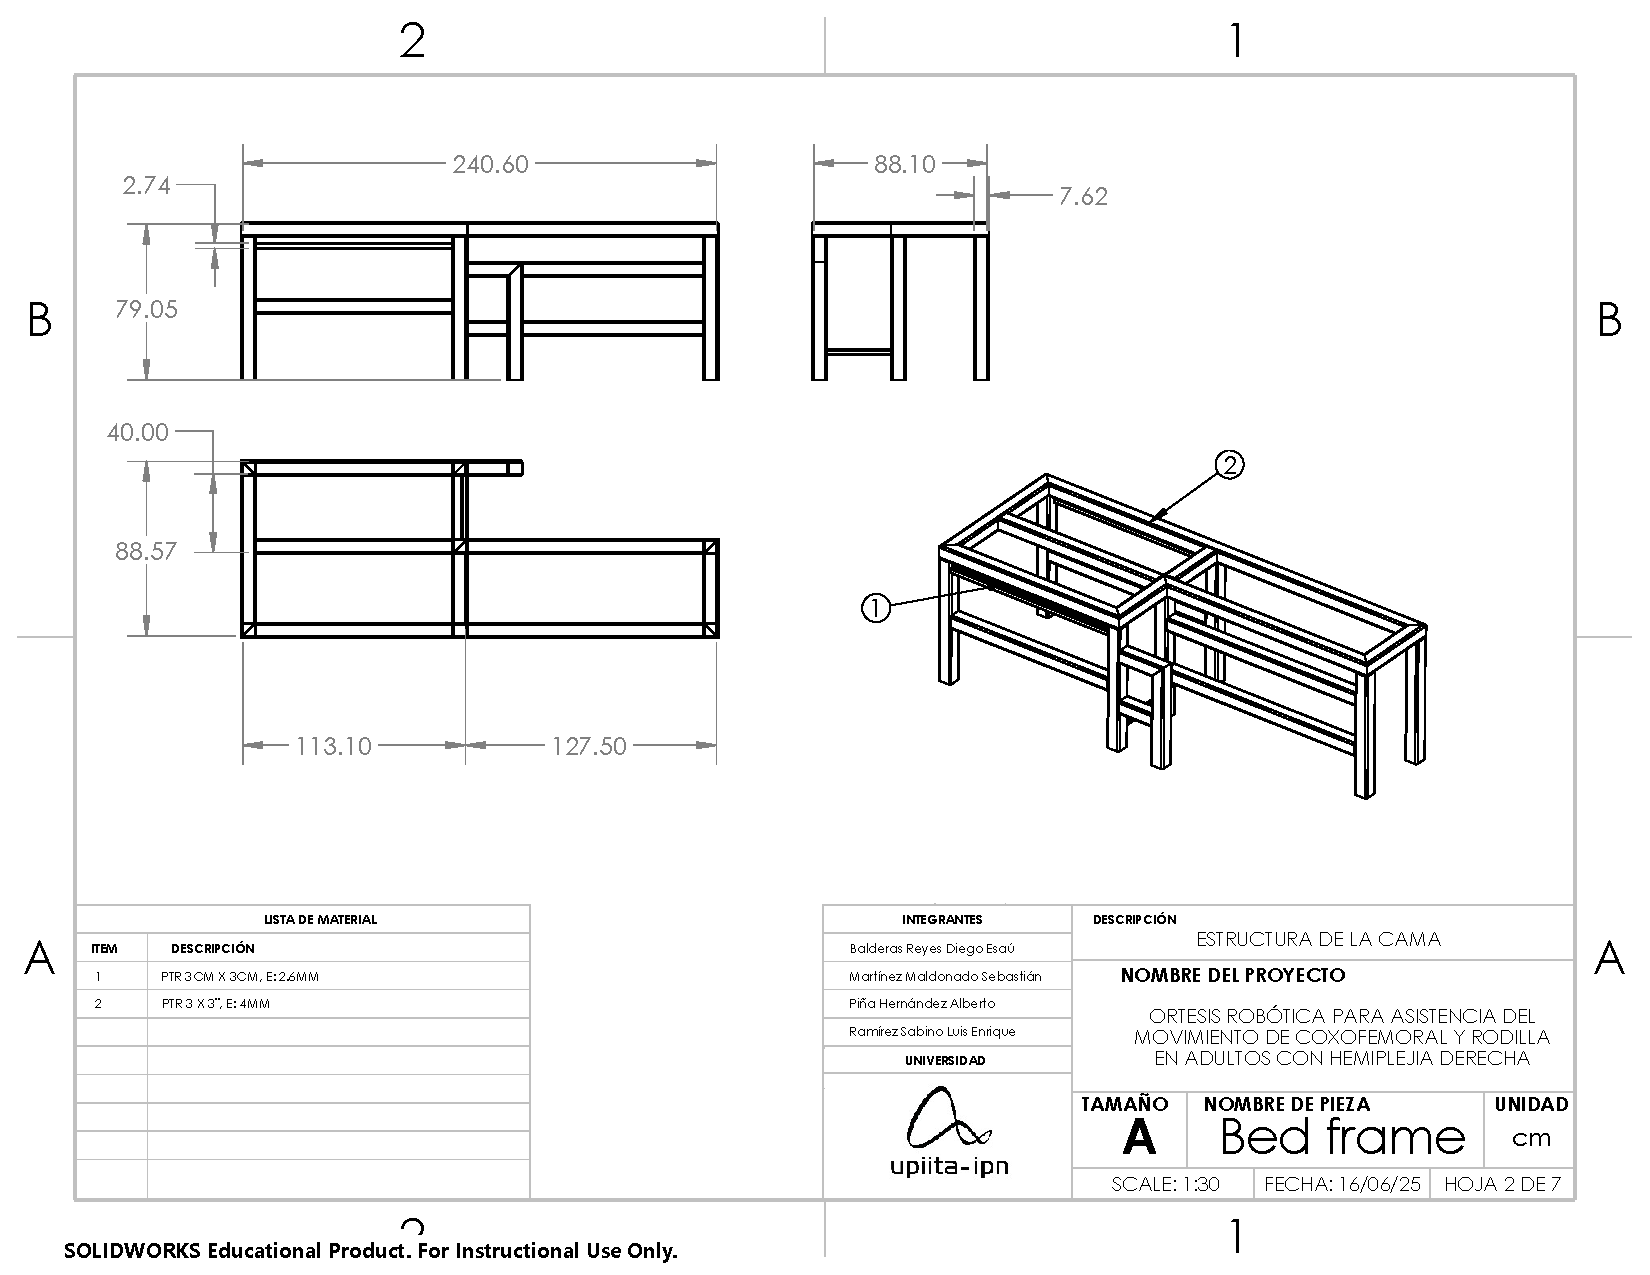
\includegraphics[trim={0 0cm 0 0},clip, angle =90, width=0.85\textwidth]{figure/planos_manufactura/horma-2.pdf}
	\caption{Estructura de la cama.}
	\label{fig:planos_estructura cama}
	\end{figure}
    \begin{figure}[h!]
	\centering
	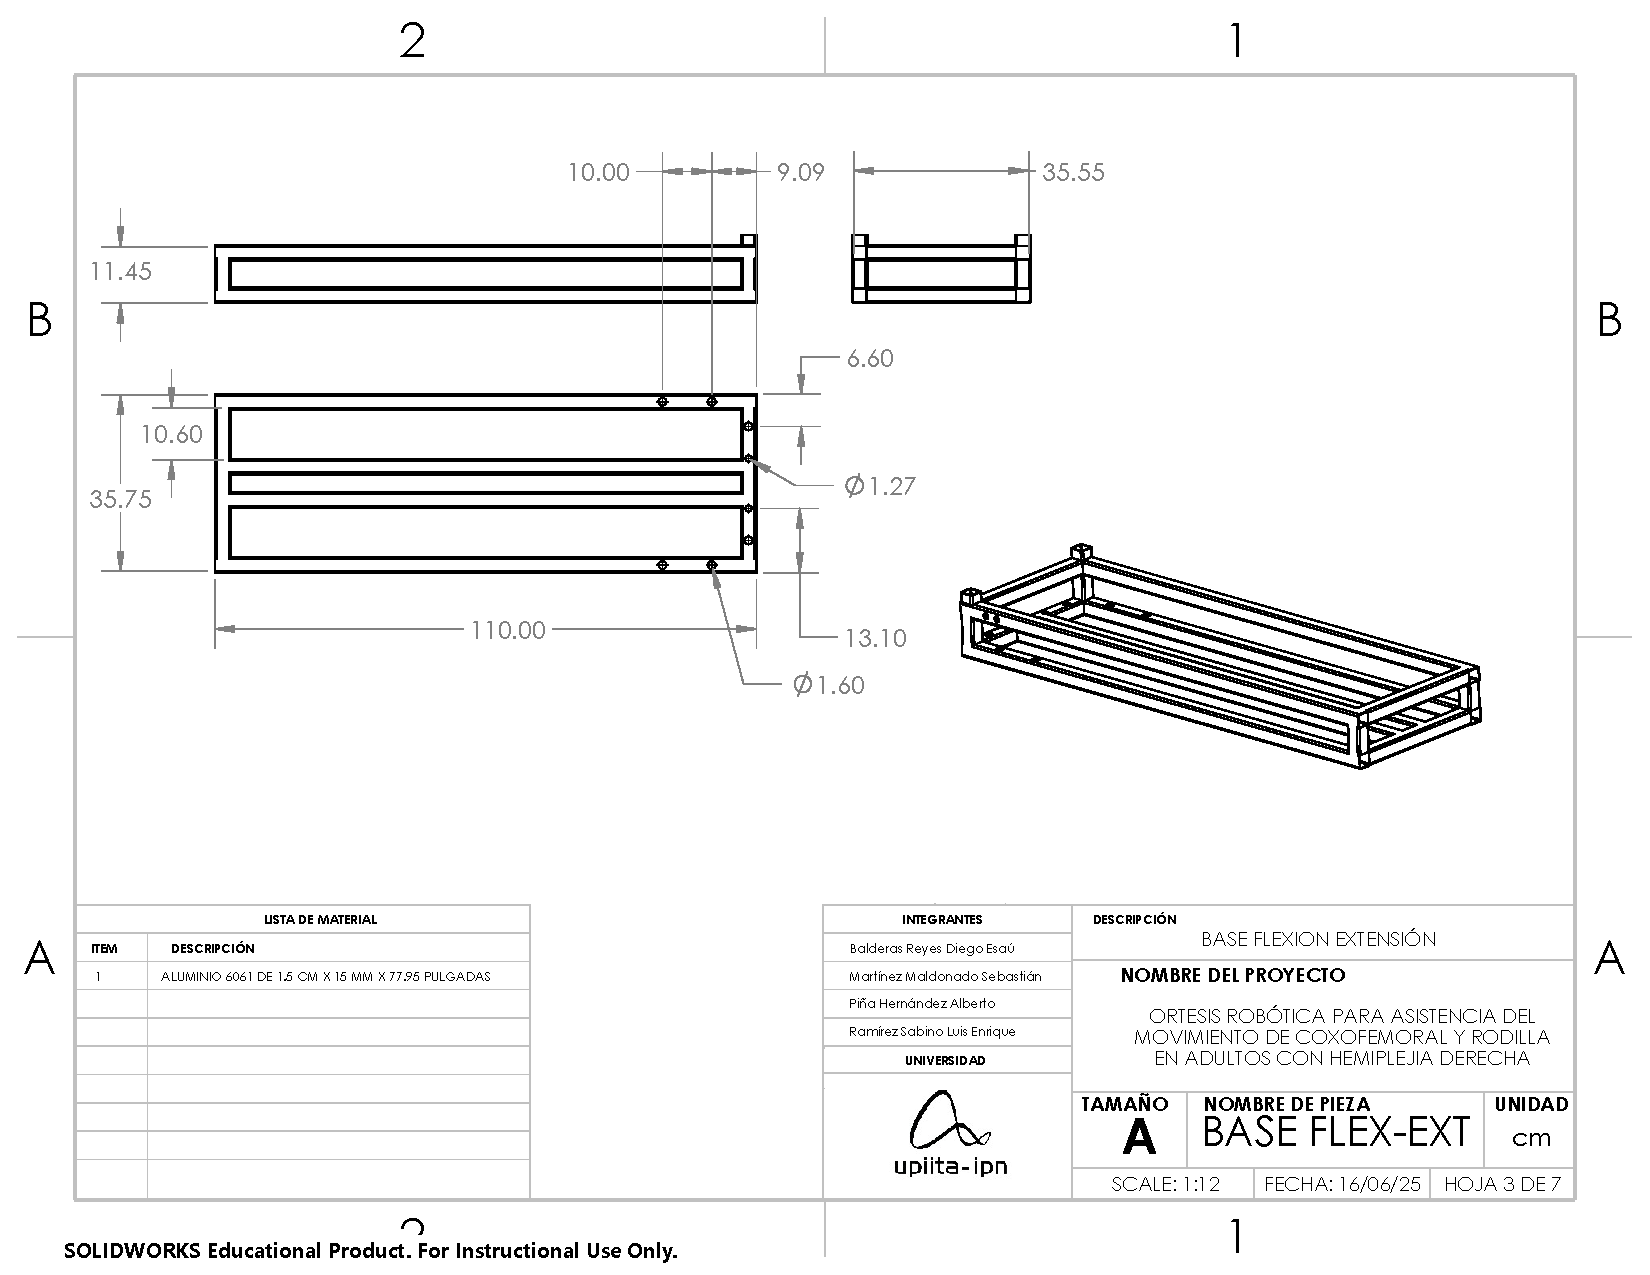
\includegraphics[trim={0 0cm 0 0},clip, angle =90, width=0.88\textwidth]{figure/planos_manufactura/horma-3.pdf}
	\caption{Base flexión-extensión.}
	\label{fig:planos_base flexion extension}
	\end{figure}
    \begin{figure}[h!]
	\centering
	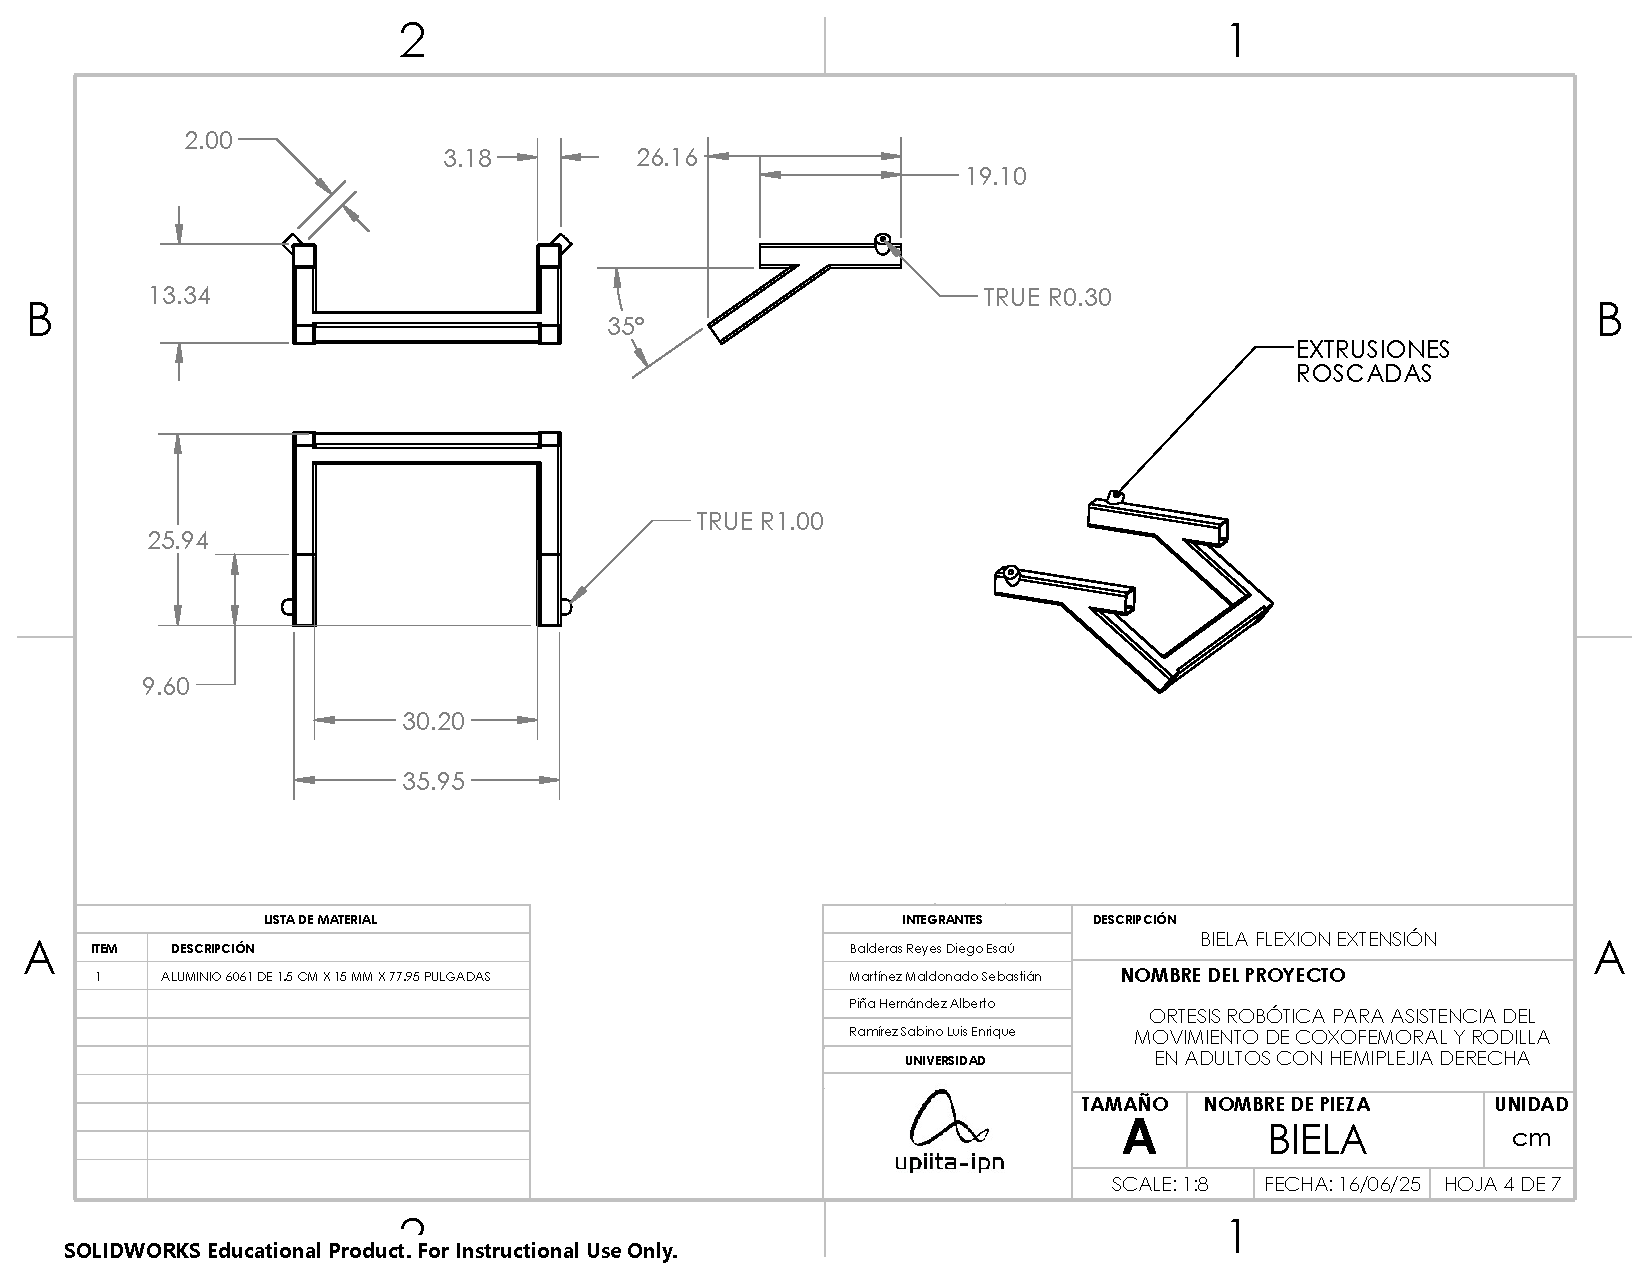
\includegraphics[trim={0 0cm 0 0},clip, angle =90, width=0.88\textwidth]{figure/planos_manufactura/horma-4.pdf}
	\caption{Biela flexión-extensión.}
	\label{fig:planos_biela flexión-extensión.}
	\end{figure}
    \begin{figure}[h!]
	\centering
	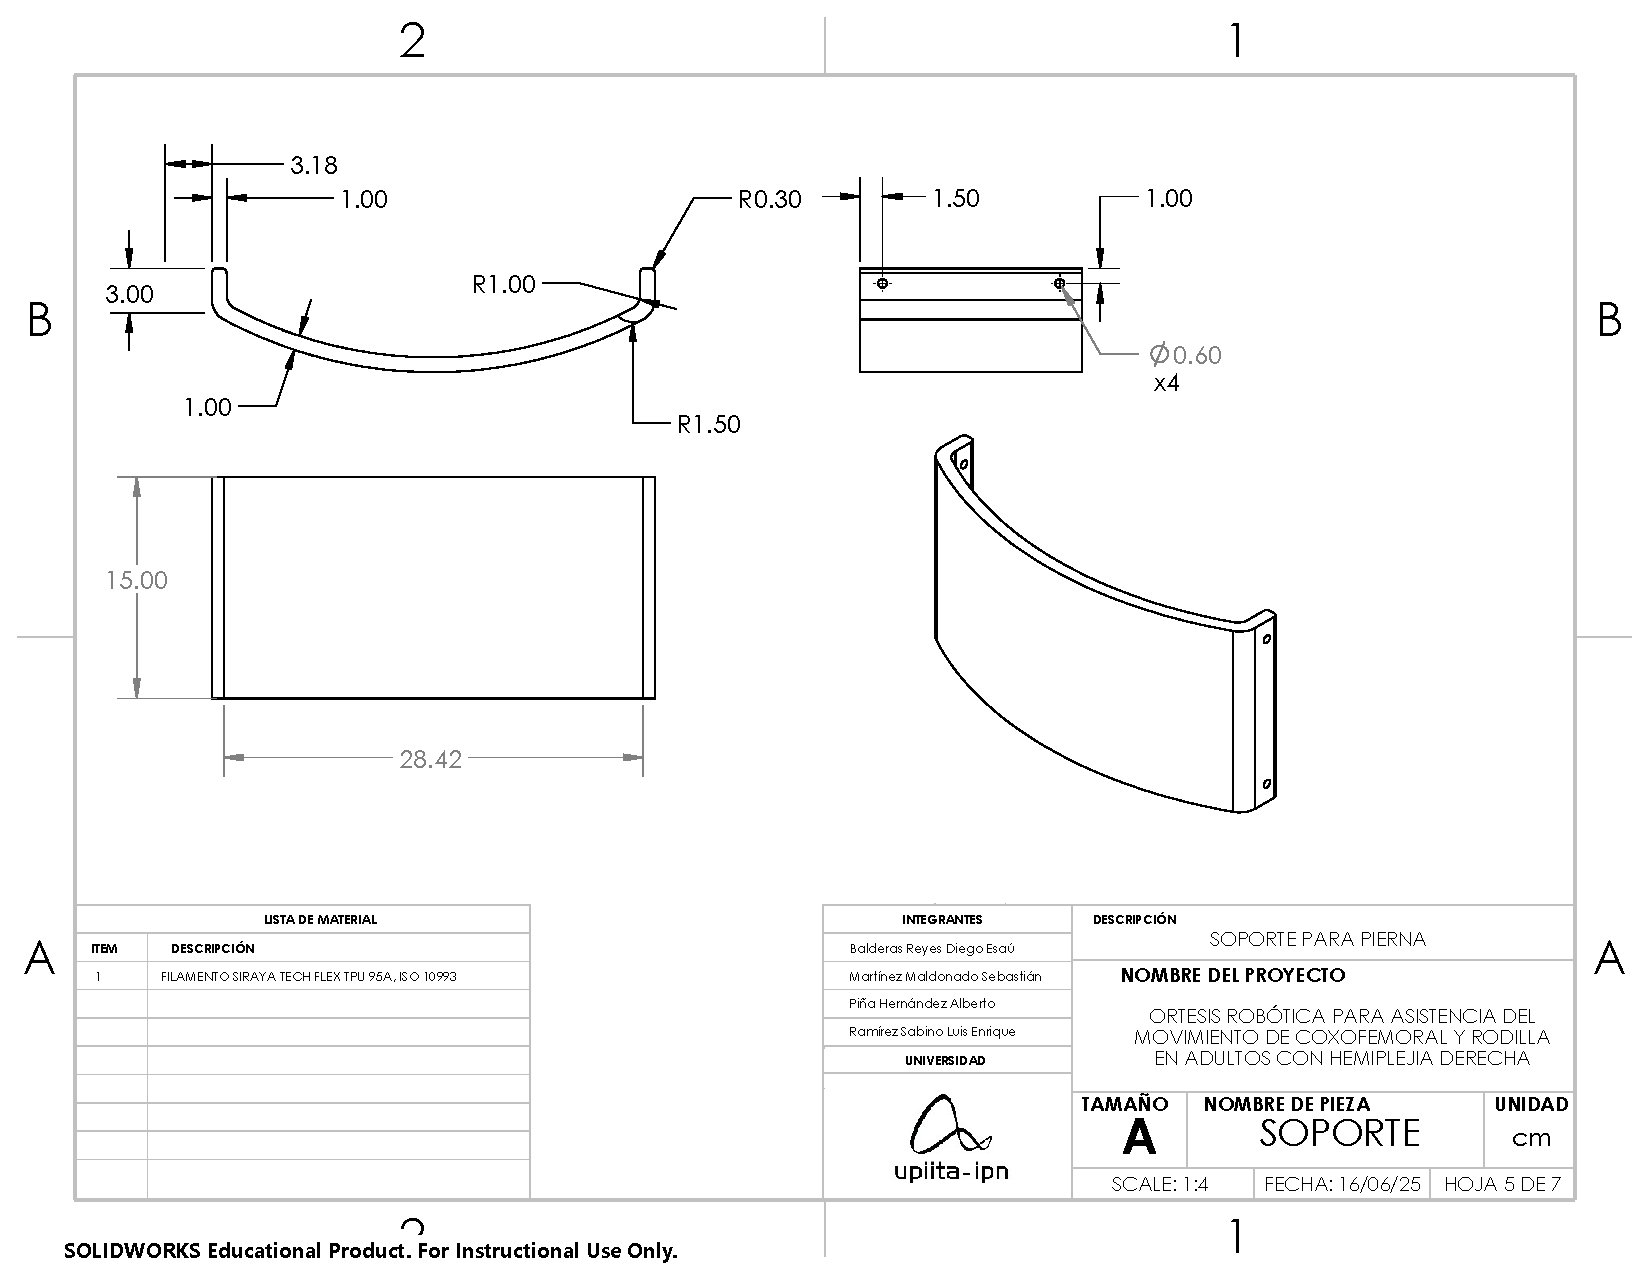
\includegraphics[trim={0 0cm 0 0},clip, angle =90, width=0.88\textwidth]{figure/planos_manufactura/horma-5.pdf}
	\caption{Soporte para pierna.}
	\label{fig:planos_soporte para pierna}
	\end{figure}
    \begin{figure}[h!]
	\centering
	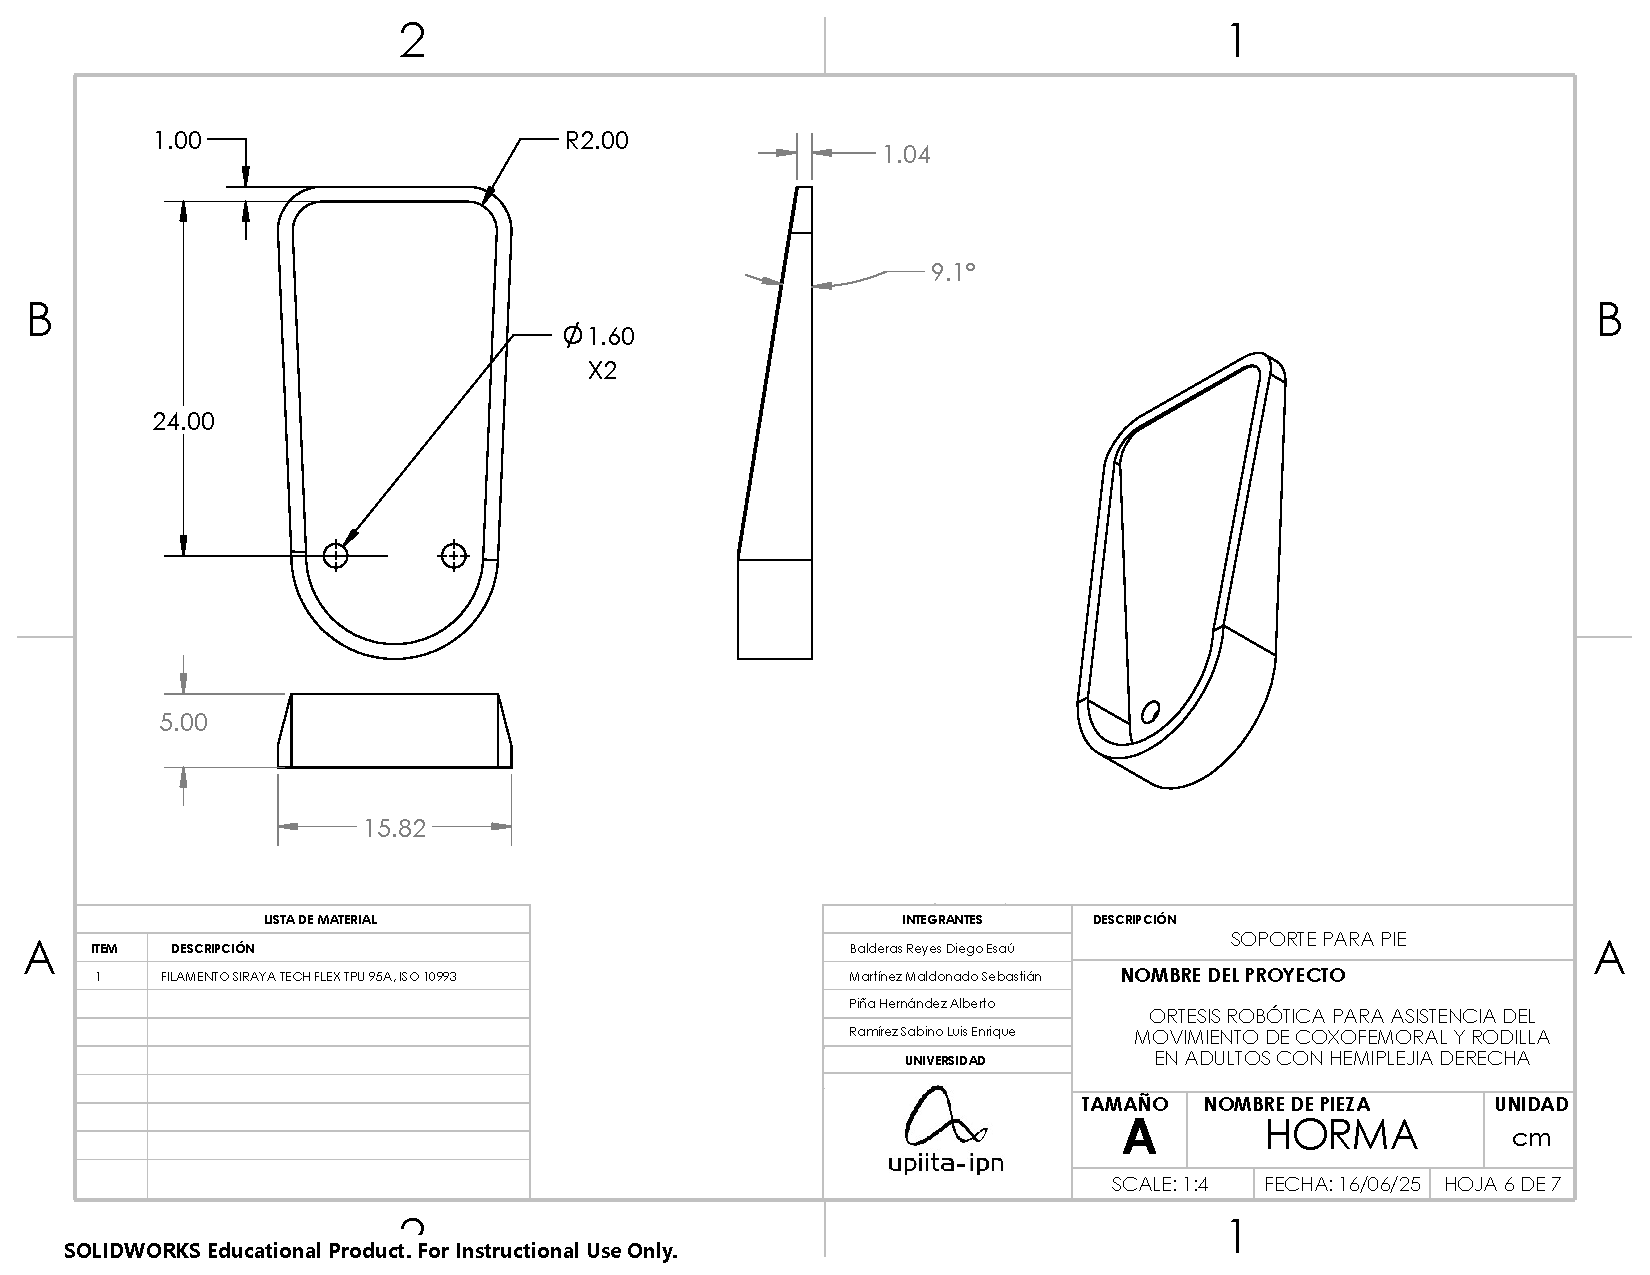
\includegraphics[trim={0 0cm 0 0},clip, angle =90, width=0.88\textwidth]{figure/planos_manufactura/horma-6.pdf}
	\caption{Soporte para pie.}
	\label{fig:planos_soporte para pie}
	\end{figure}
    \begin{figure}[h!]
	\centering
	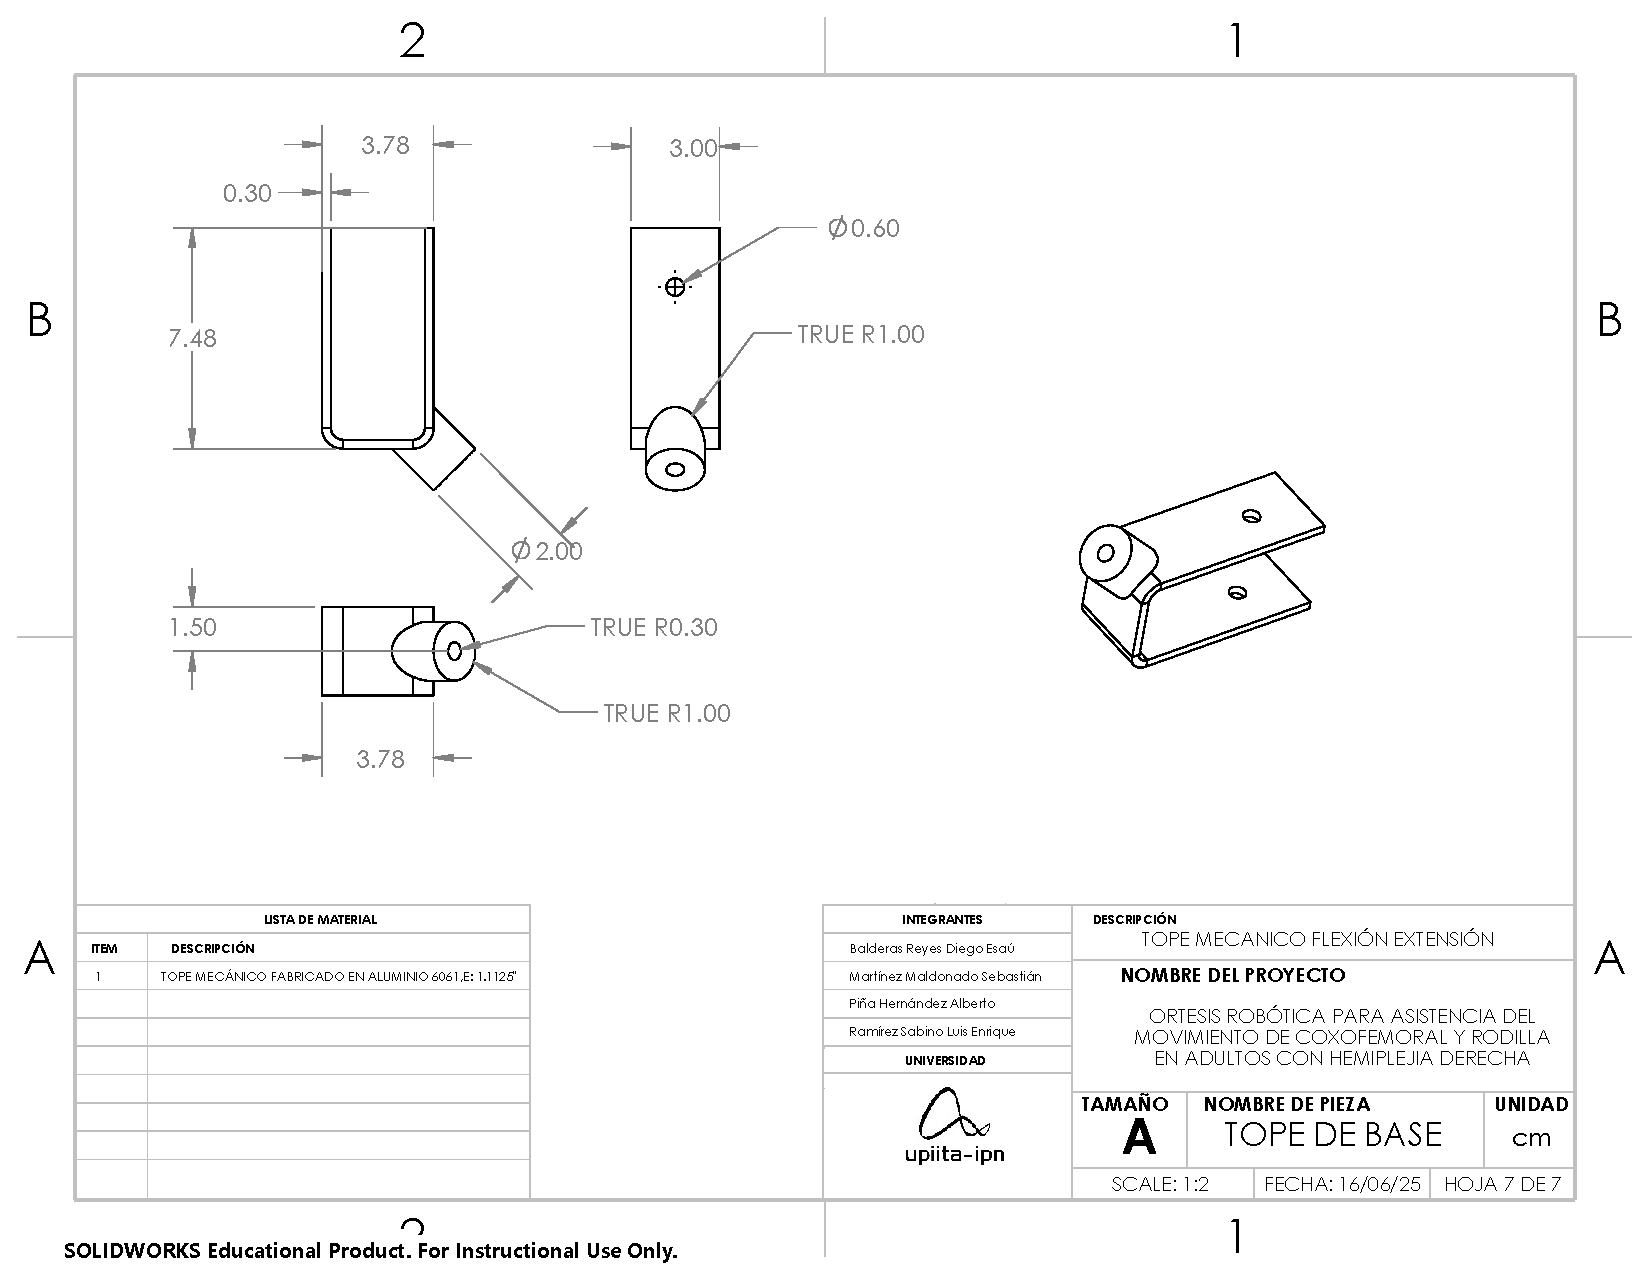
\includegraphics[trim={0 0cm 0 0},clip, angle =90, width=0.88\textwidth]{figure/planos_manufactura/horma-7.pdf}
	\caption{Tope mecánico de flexión-extensión.}
	\label{fig:planos_tope mecánico de flexión-extensión}
	\end{figure}

    \begin{figure}[h!]
	\centering
	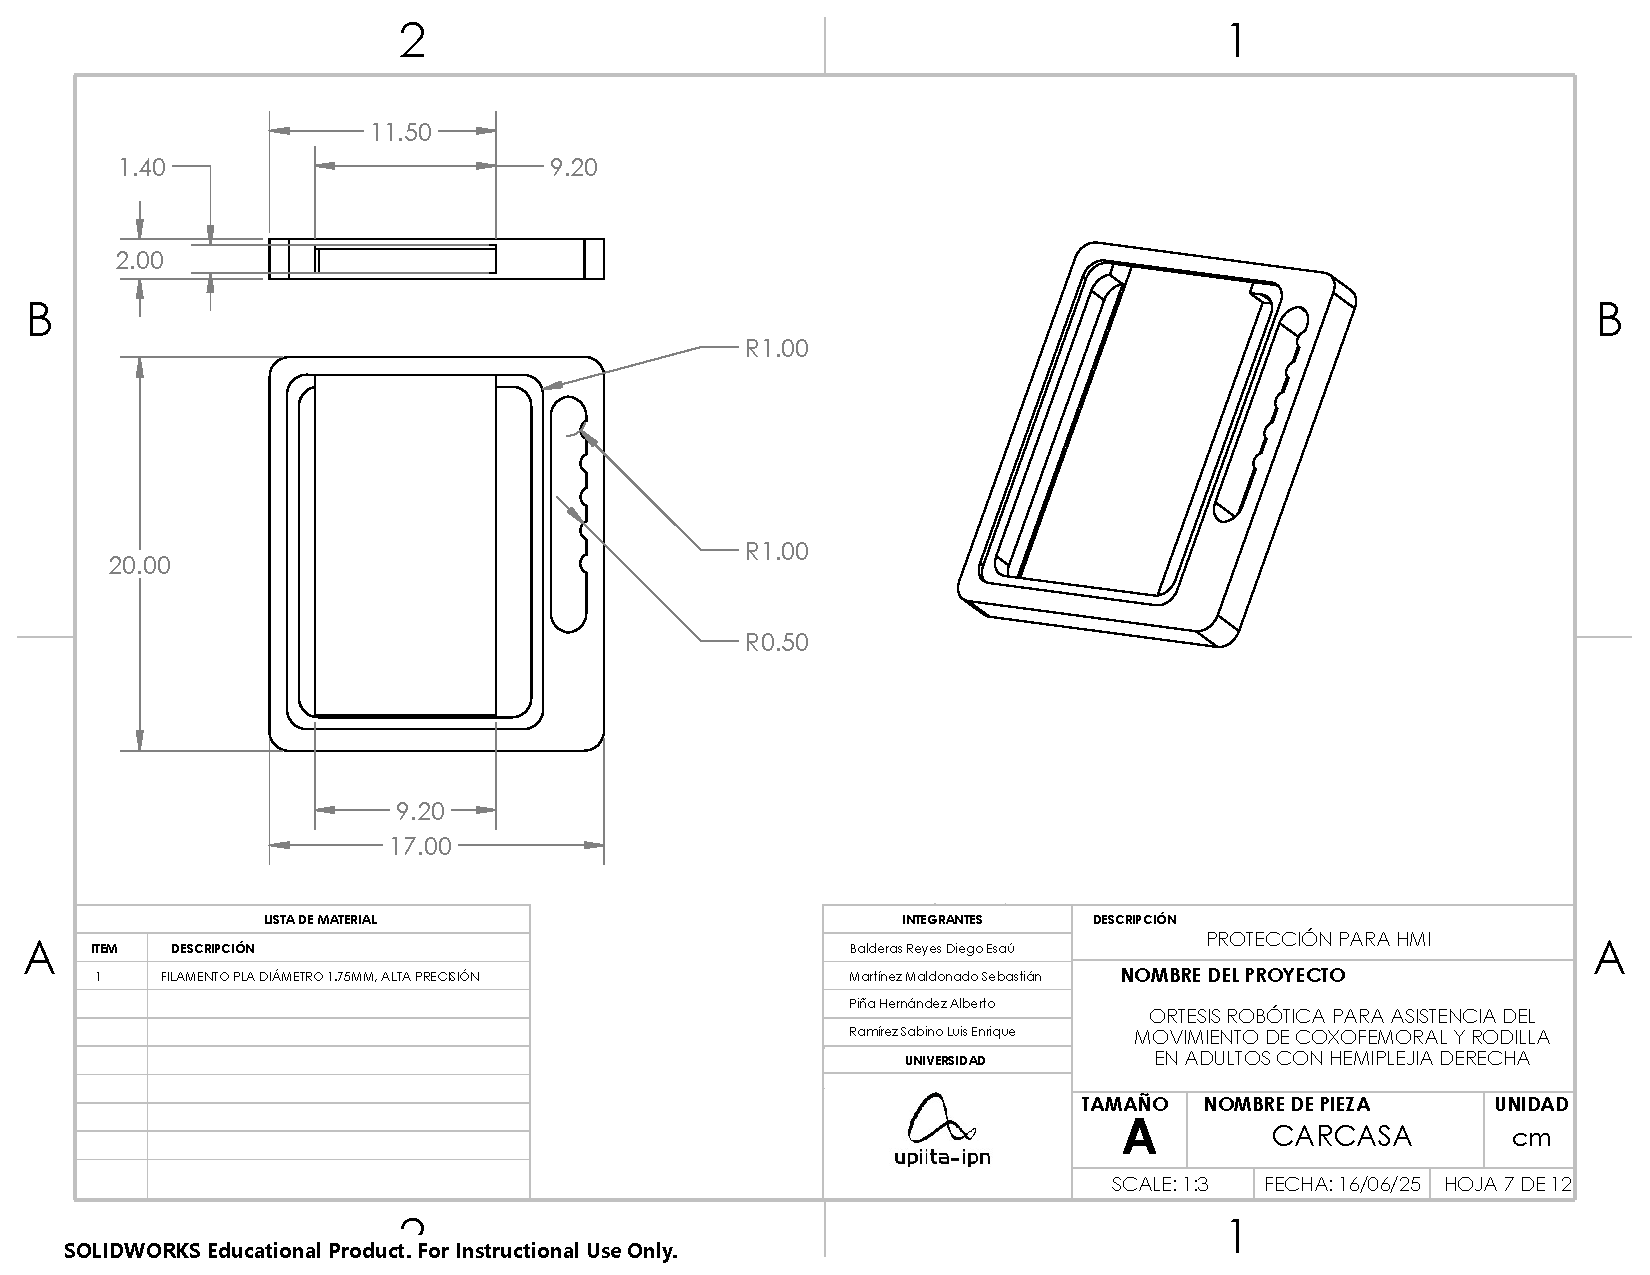
\includegraphics[trim={0 0cm 0 0},clip, angle =90, width=0.88\textwidth]{figure/planos_manufactura/Planos-7-12-1.pdf}
	\caption{Protección para HMI.}
	\label{fig:planos_protección para hmi}
	\end{figure}
    \begin{figure}[h!]
	\centering
	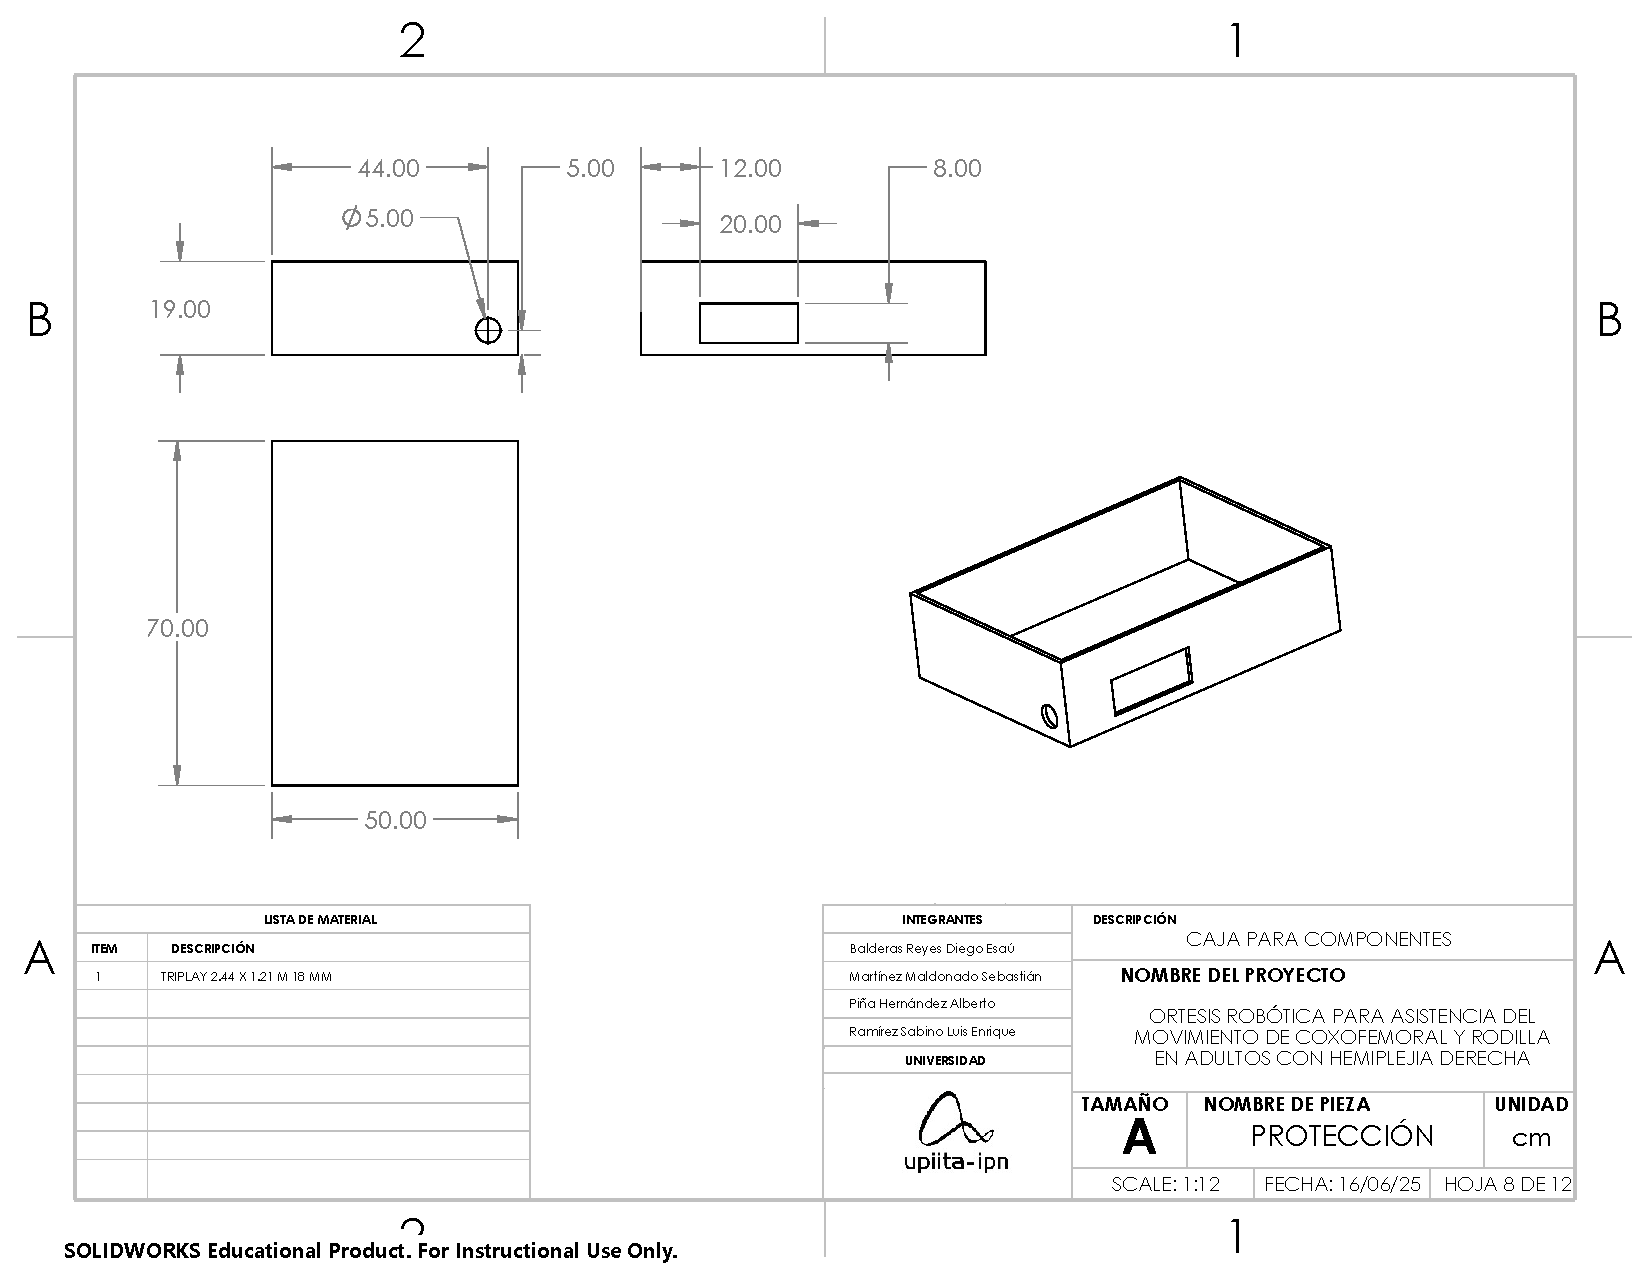
\includegraphics[trim={0 0cm 0 0},clip, angle =90, width=0.88\textwidth]{figure/planos_manufactura/Planos-7-12-2.pdf}
	\caption{Caja para componentes.}
	\label{fig:planos_caja para componentes}
	\end{figure}
    \begin{figure}[h!]
	\centering
	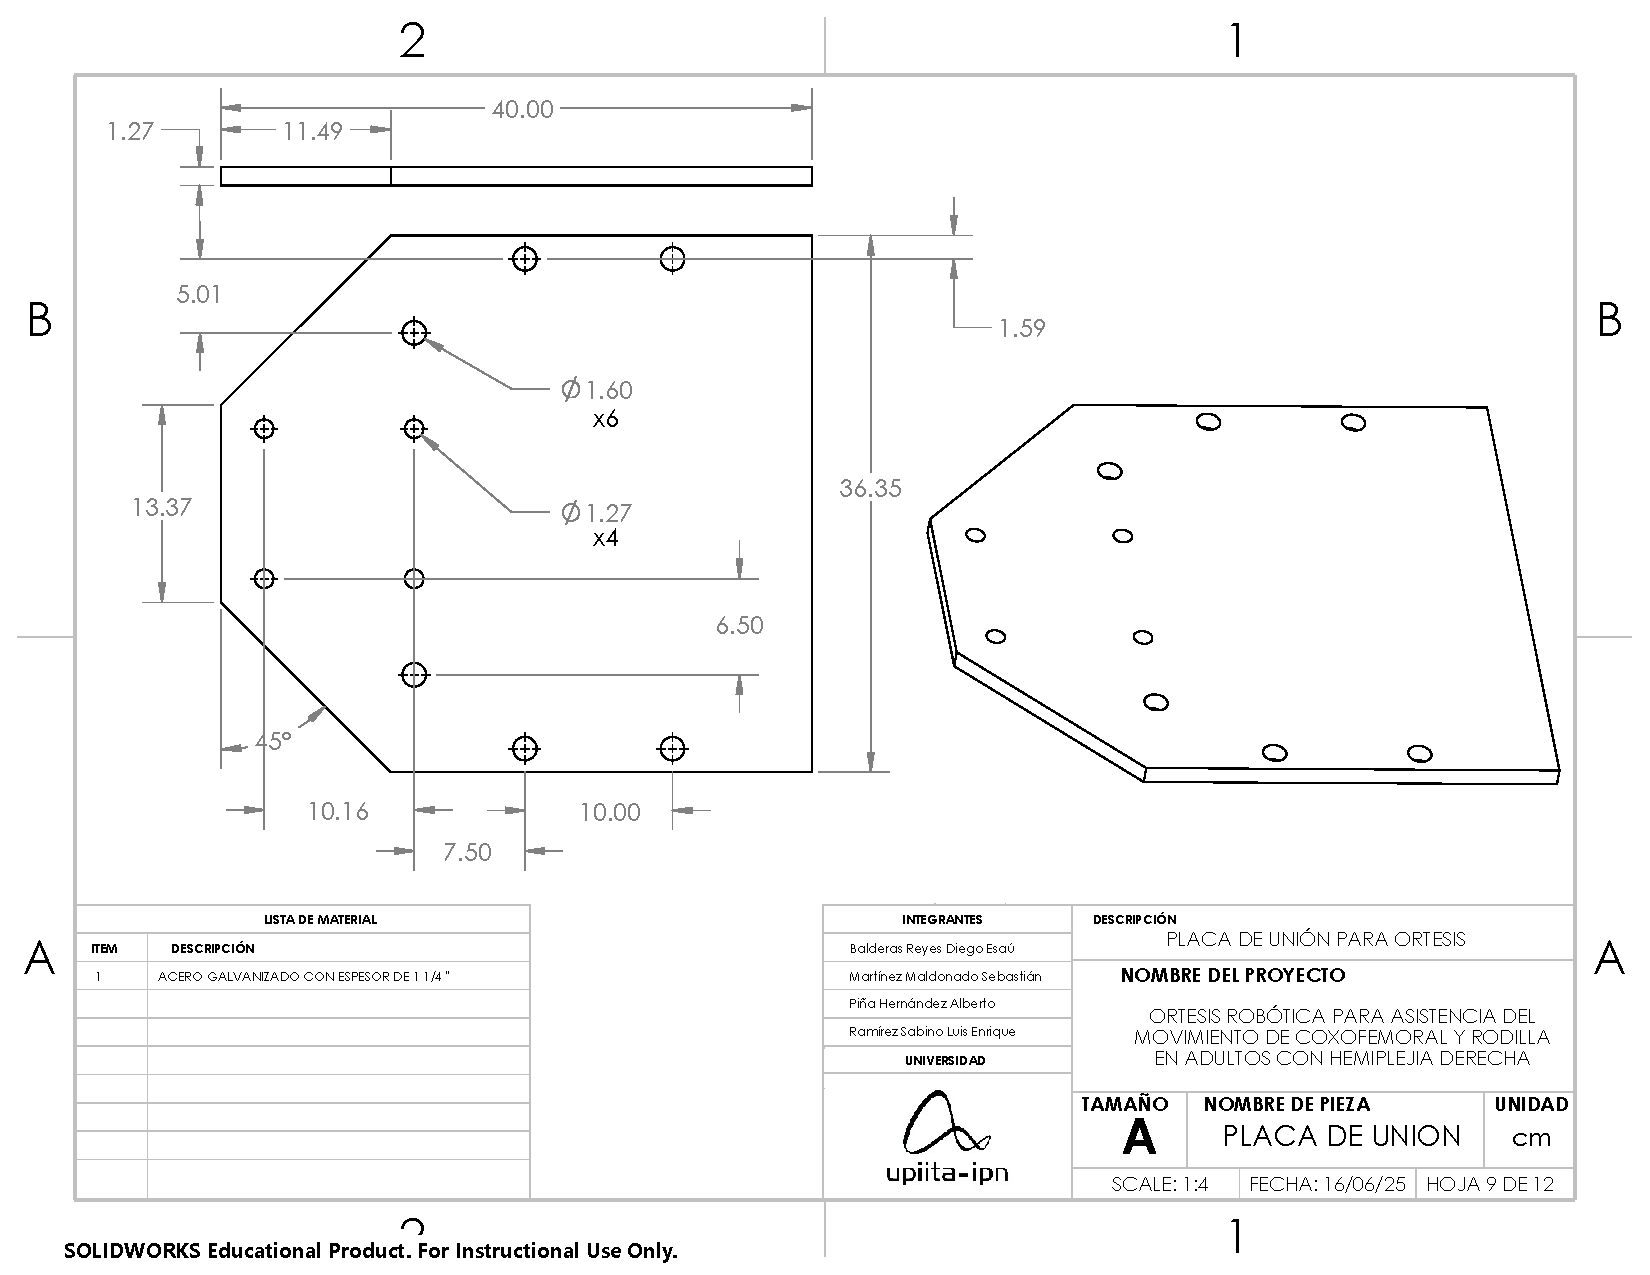
\includegraphics[trim={0 0cm 0 0},clip, angle =90, width=0.88\textwidth]{figure/planos_manufactura/Planos-7-12-3.pdf}
	\caption{Placa para unión de ortesis.}
	\label{fig:planos_placa para unión de ortesis}
	\end{figure}
    \begin{figure}[h!]
	\centering
	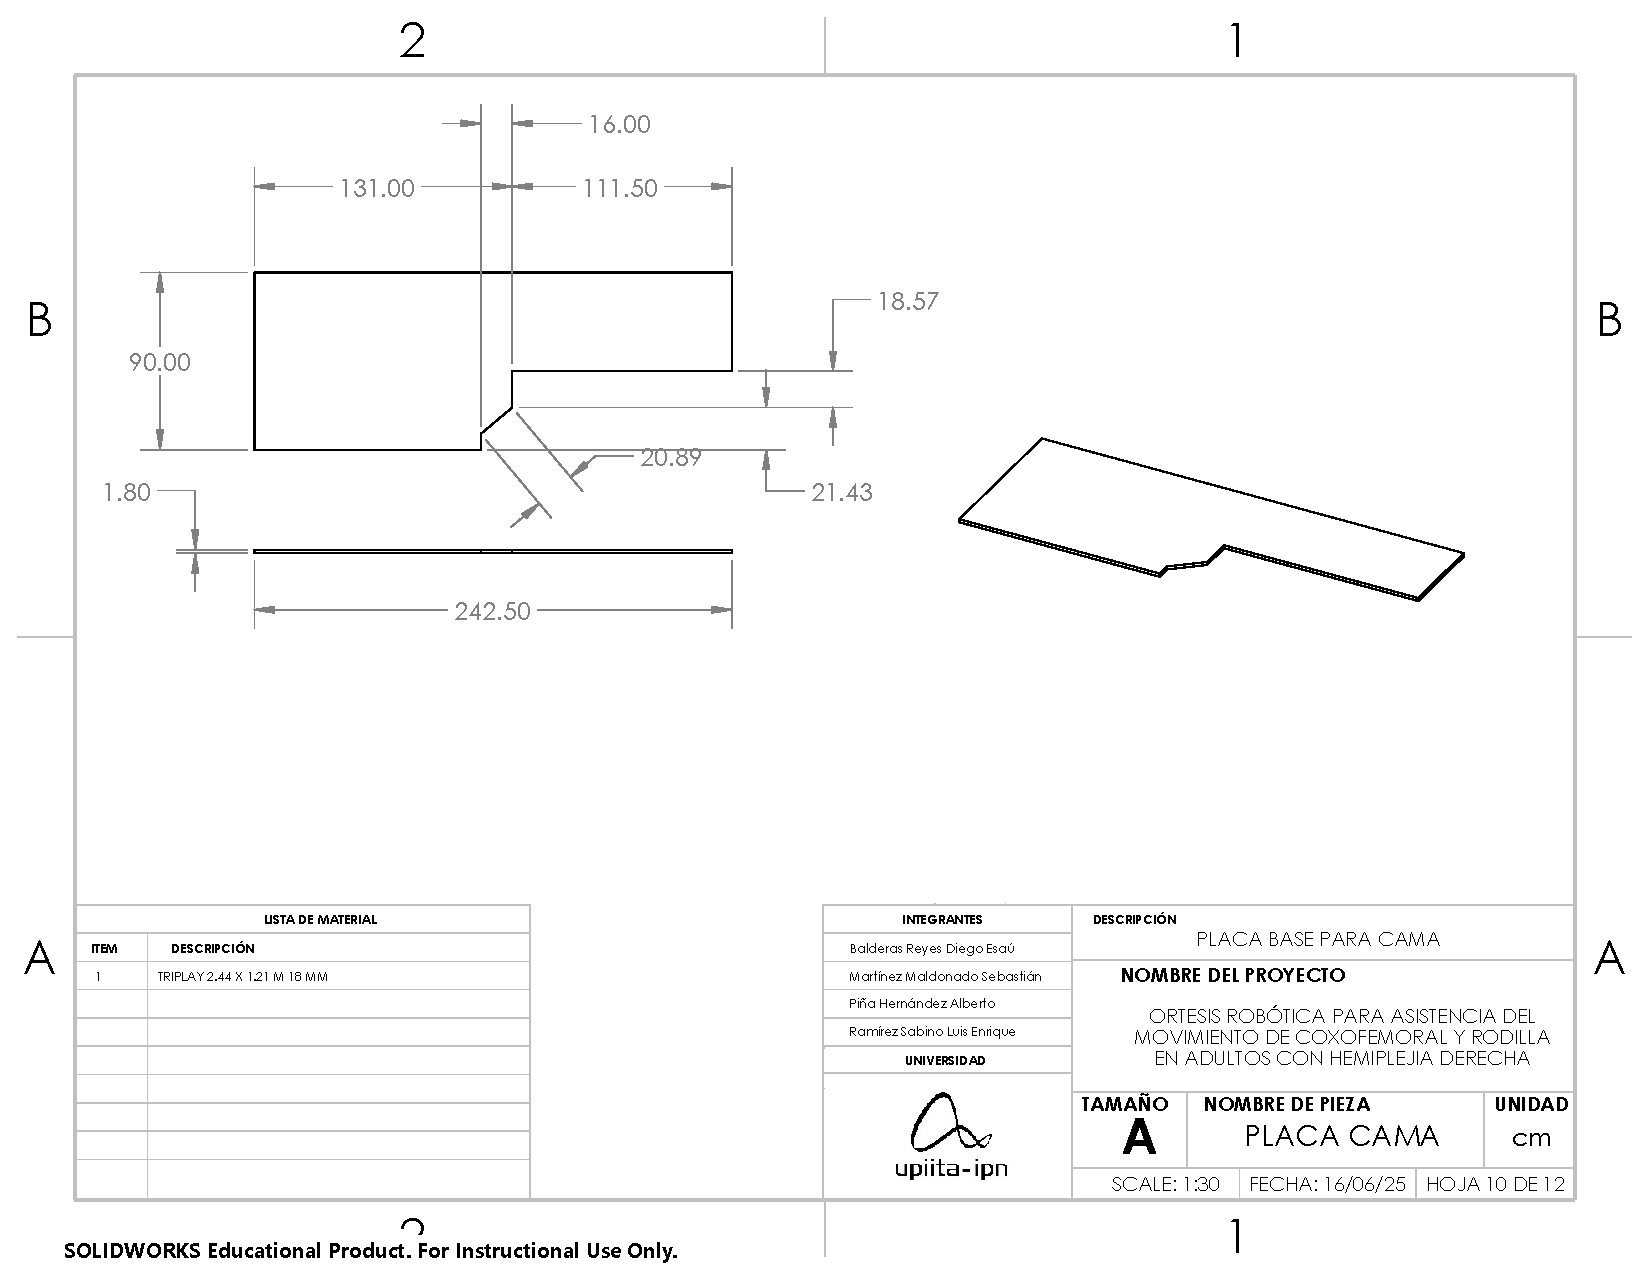
\includegraphics[trim={0 0cm 0 0},clip, angle =90, width=0.88\textwidth]{figure/planos_manufactura/Planos-7-12-4.pdf}
	\caption{Protección para HMI.}
	\label{fig:planos_protección para HMI}
	\end{figure}
    \begin{figure}[h!]
	\centering
	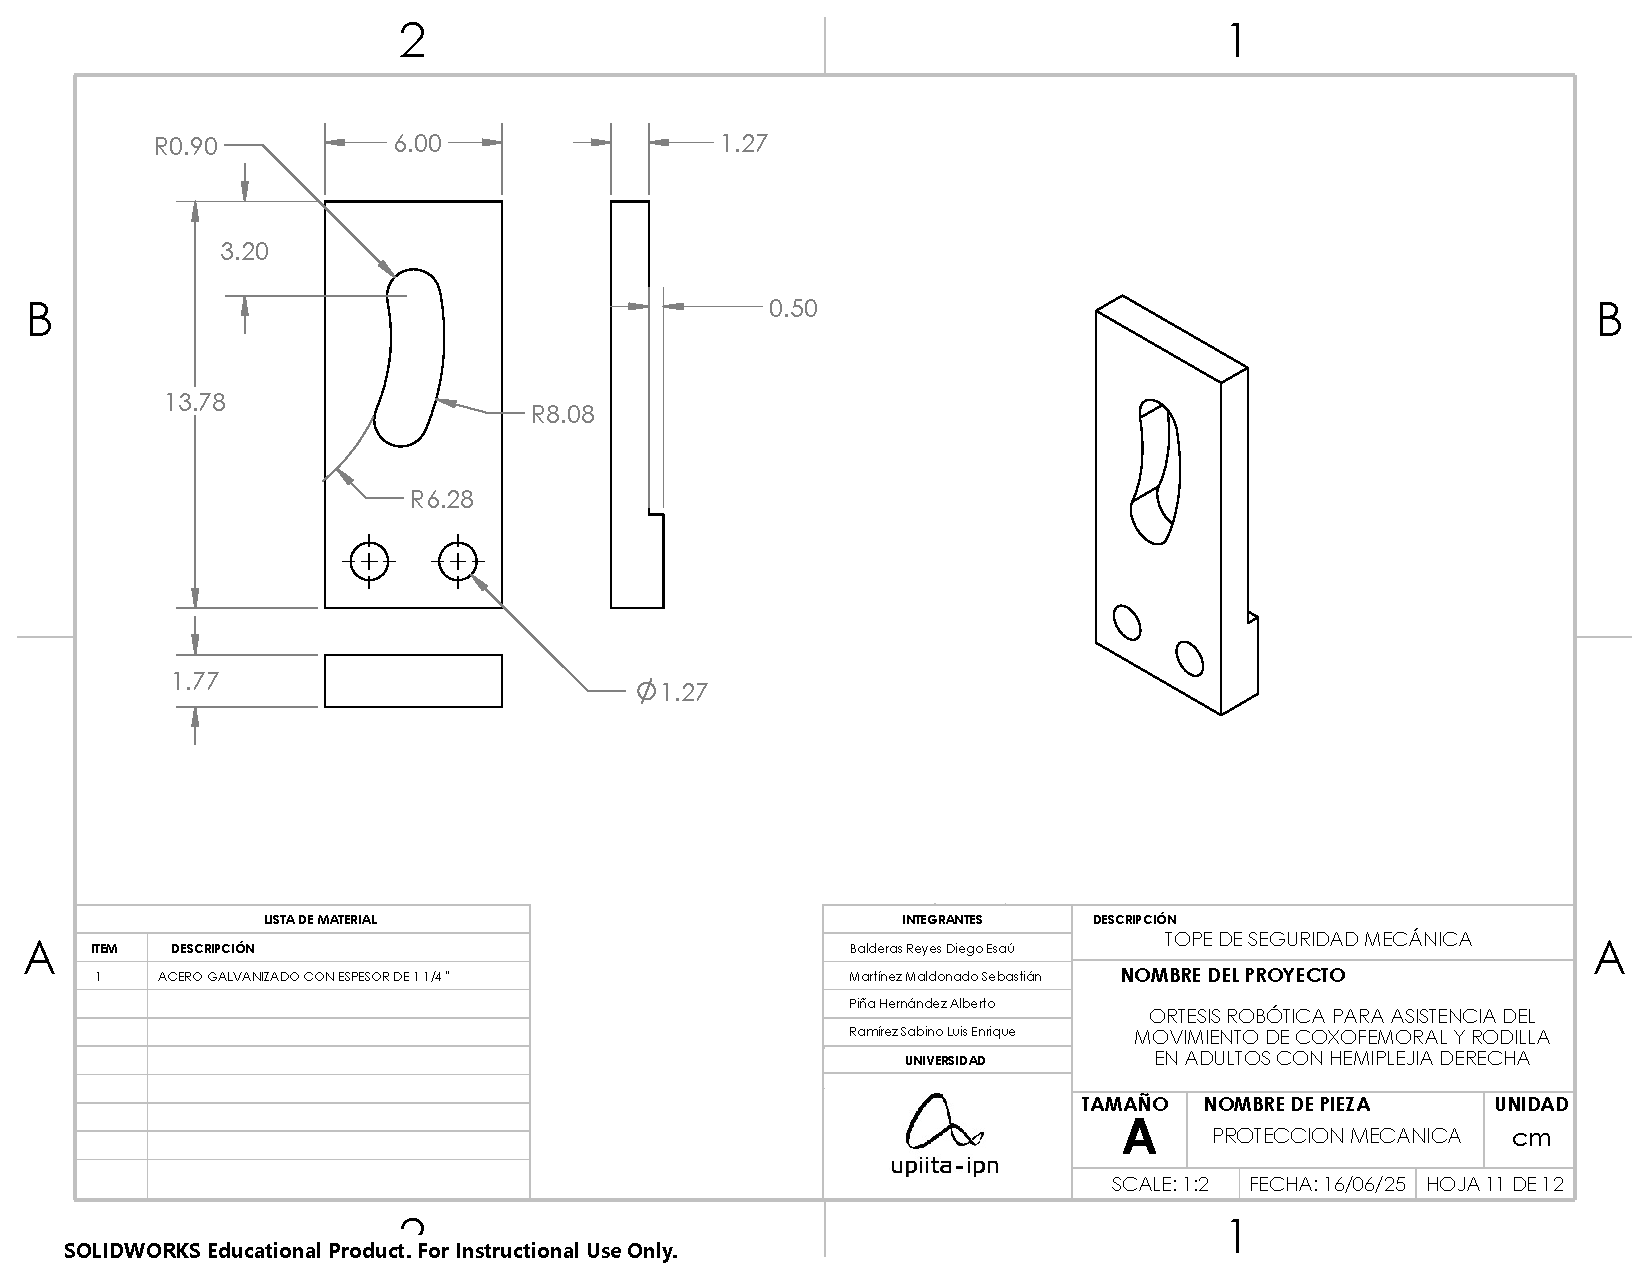
\includegraphics[trim={0 0cm 0 0},clip, angle =90, width=0.88\textwidth]{figure/planos_manufactura/Planos-7-12-5.pdf}
	\caption{Placa base para cama.}
	\label{fig:planos_placa base para cama}
	\end{figure}




    
    
    \begin{figure}[h!]
	\centering
	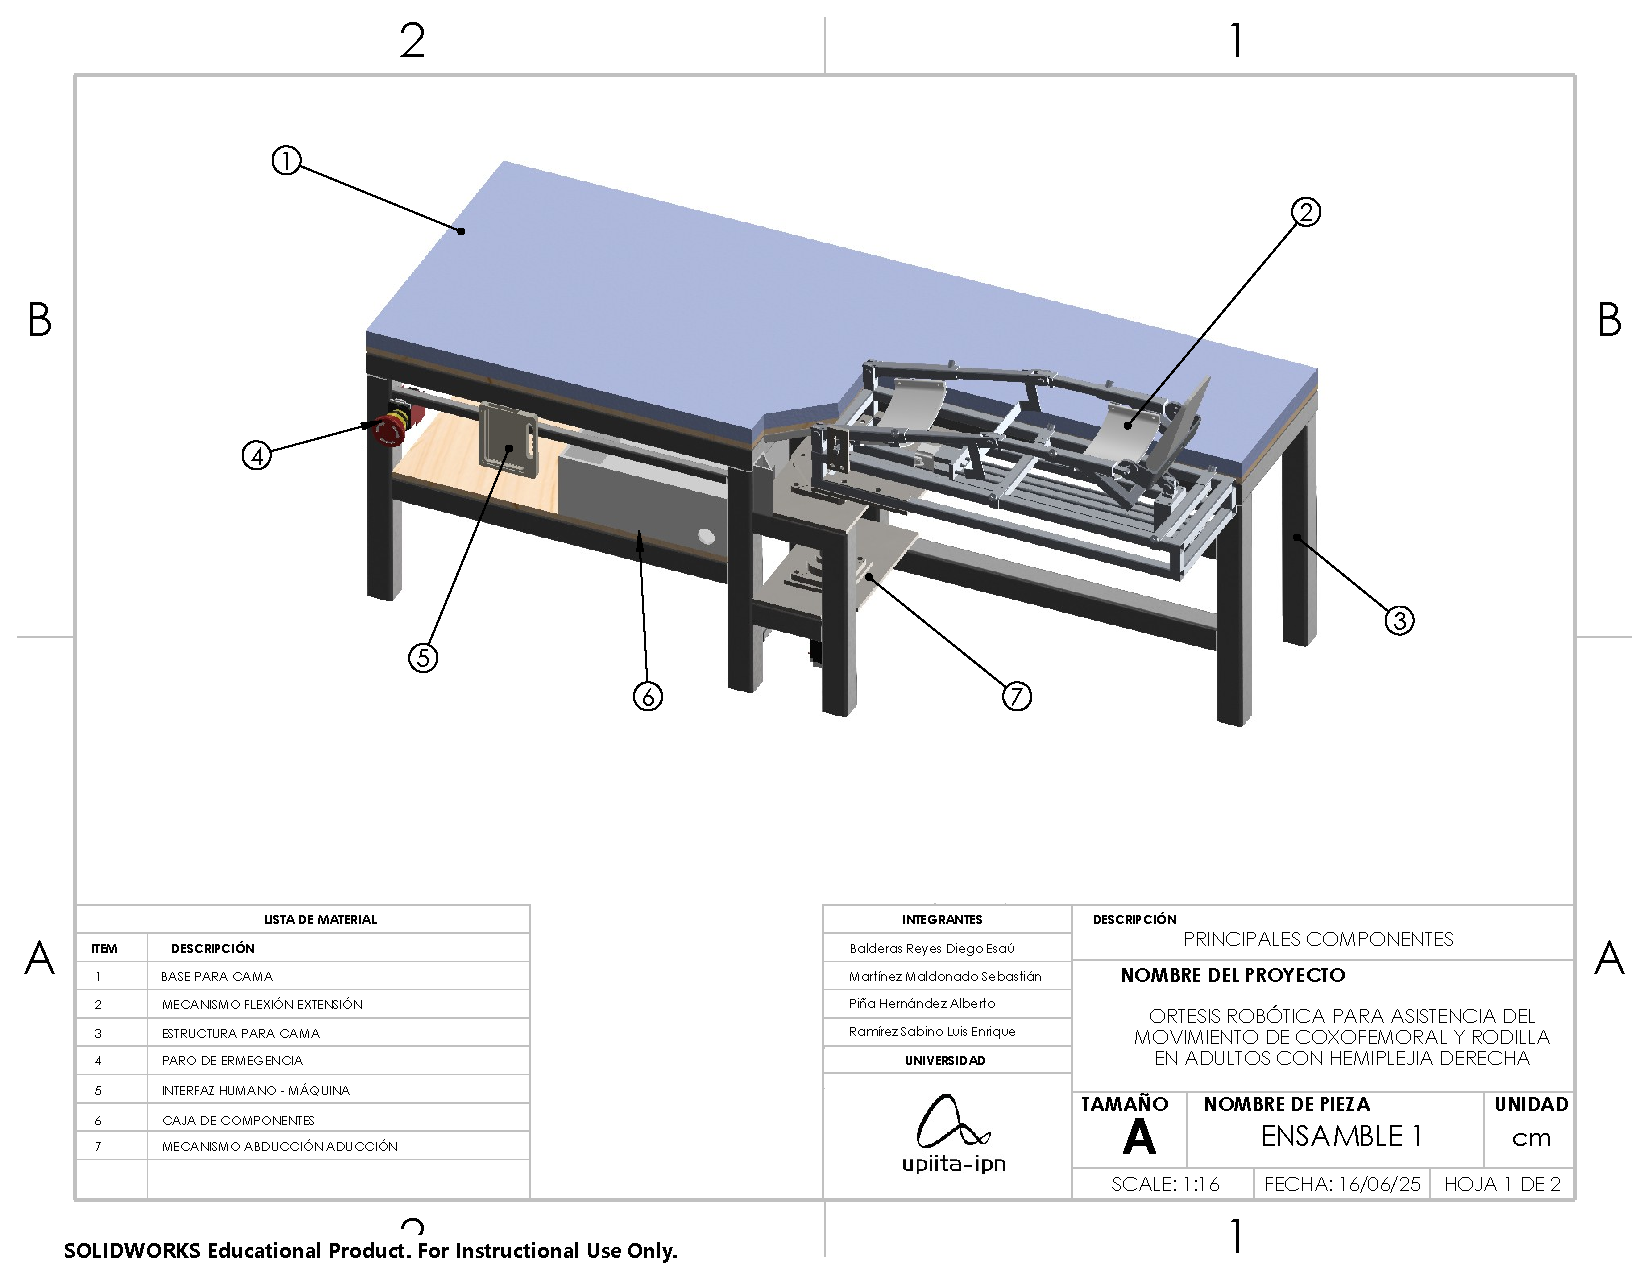
\includegraphics[trim={0 0cm 0 0},clip, angle =90, width=0.88\textwidth]{figure/planos_manufactura/Planos finales-1.pdf}
	\caption{Ensamble del proyecto - Primera parte.}
	\label{fig:plano final 1}
	\end{figure}

    \begin{figure}[h!]
	\centering
	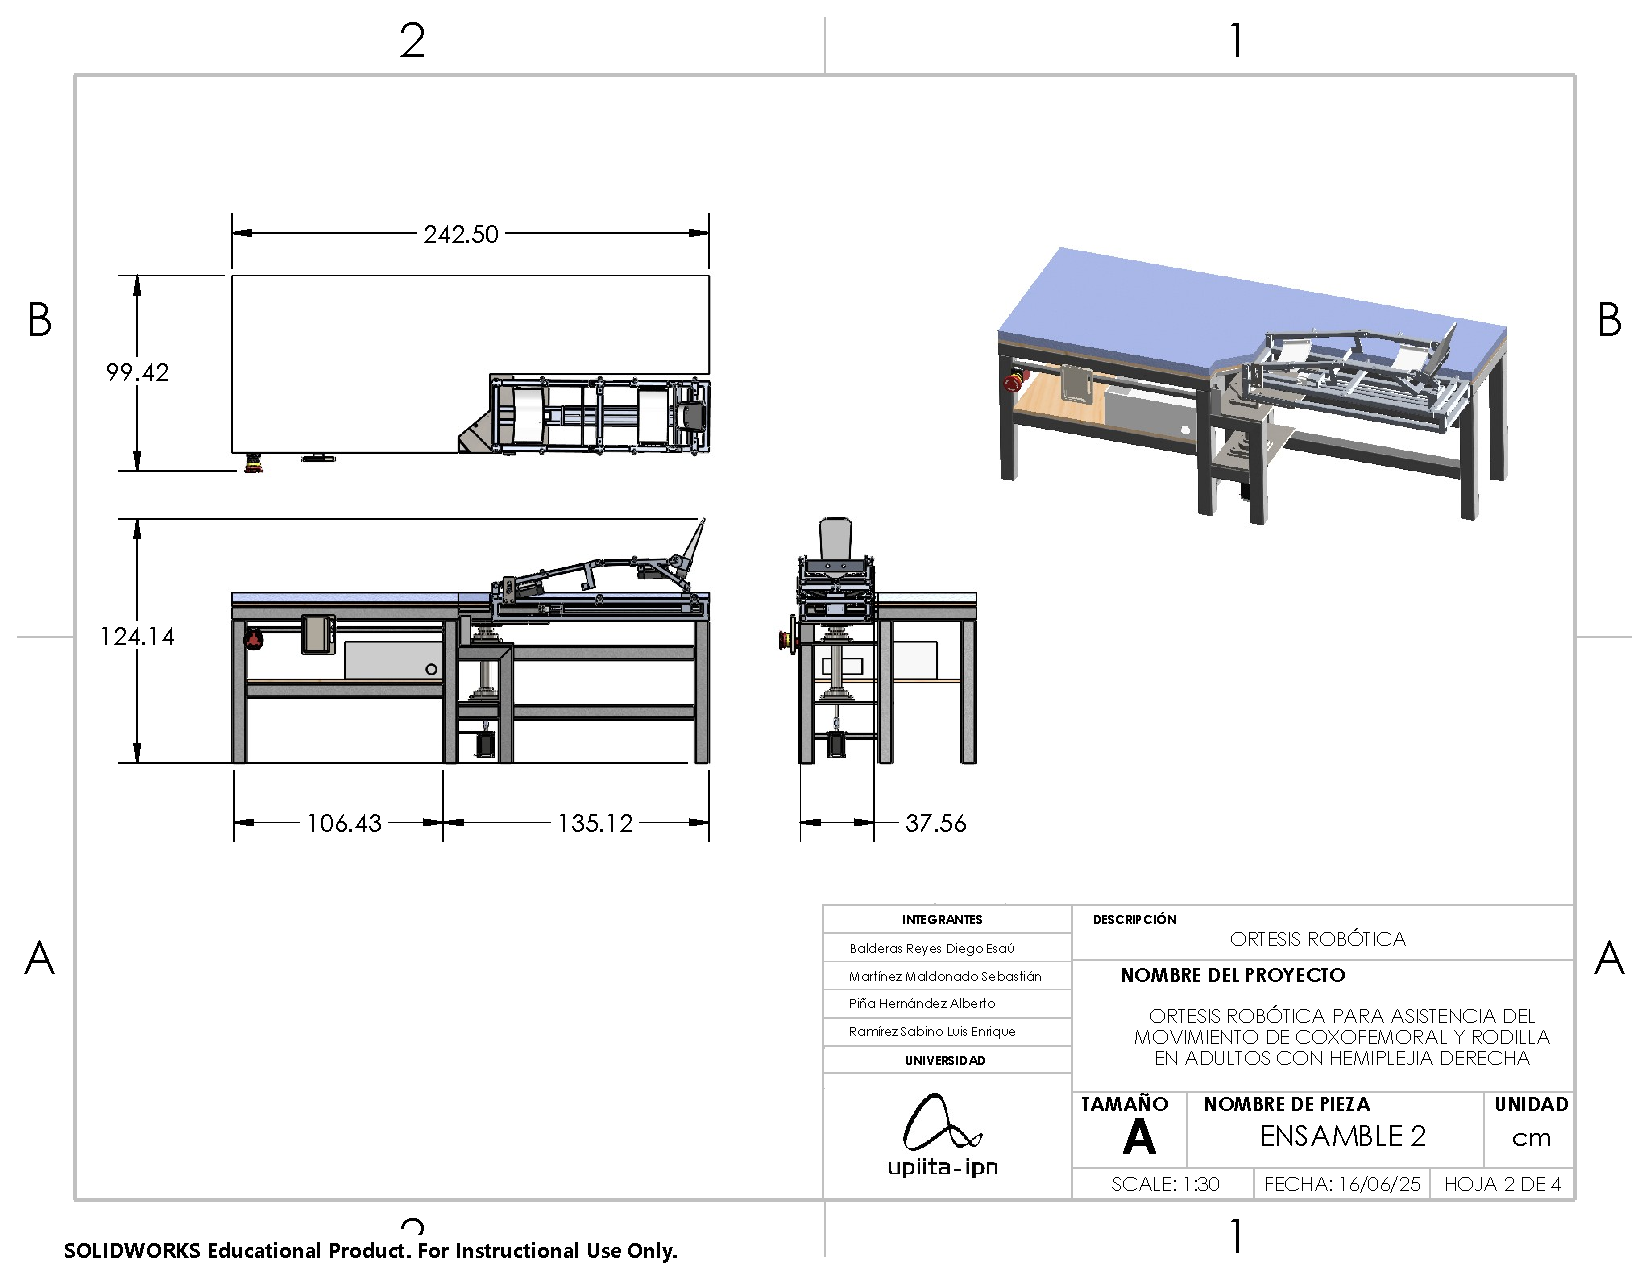
\includegraphics[trim={0 0cm 0 0},clip, angle =90, width=0.88\textwidth]{figure/planos_manufactura/Planos finales-2.pdf}
	\caption{Ensamble del proyecto - Segunda parte.}
	\label{fig:plano final 2}
	\end{figure}
    \begin{figure}[h!]
	\centering
	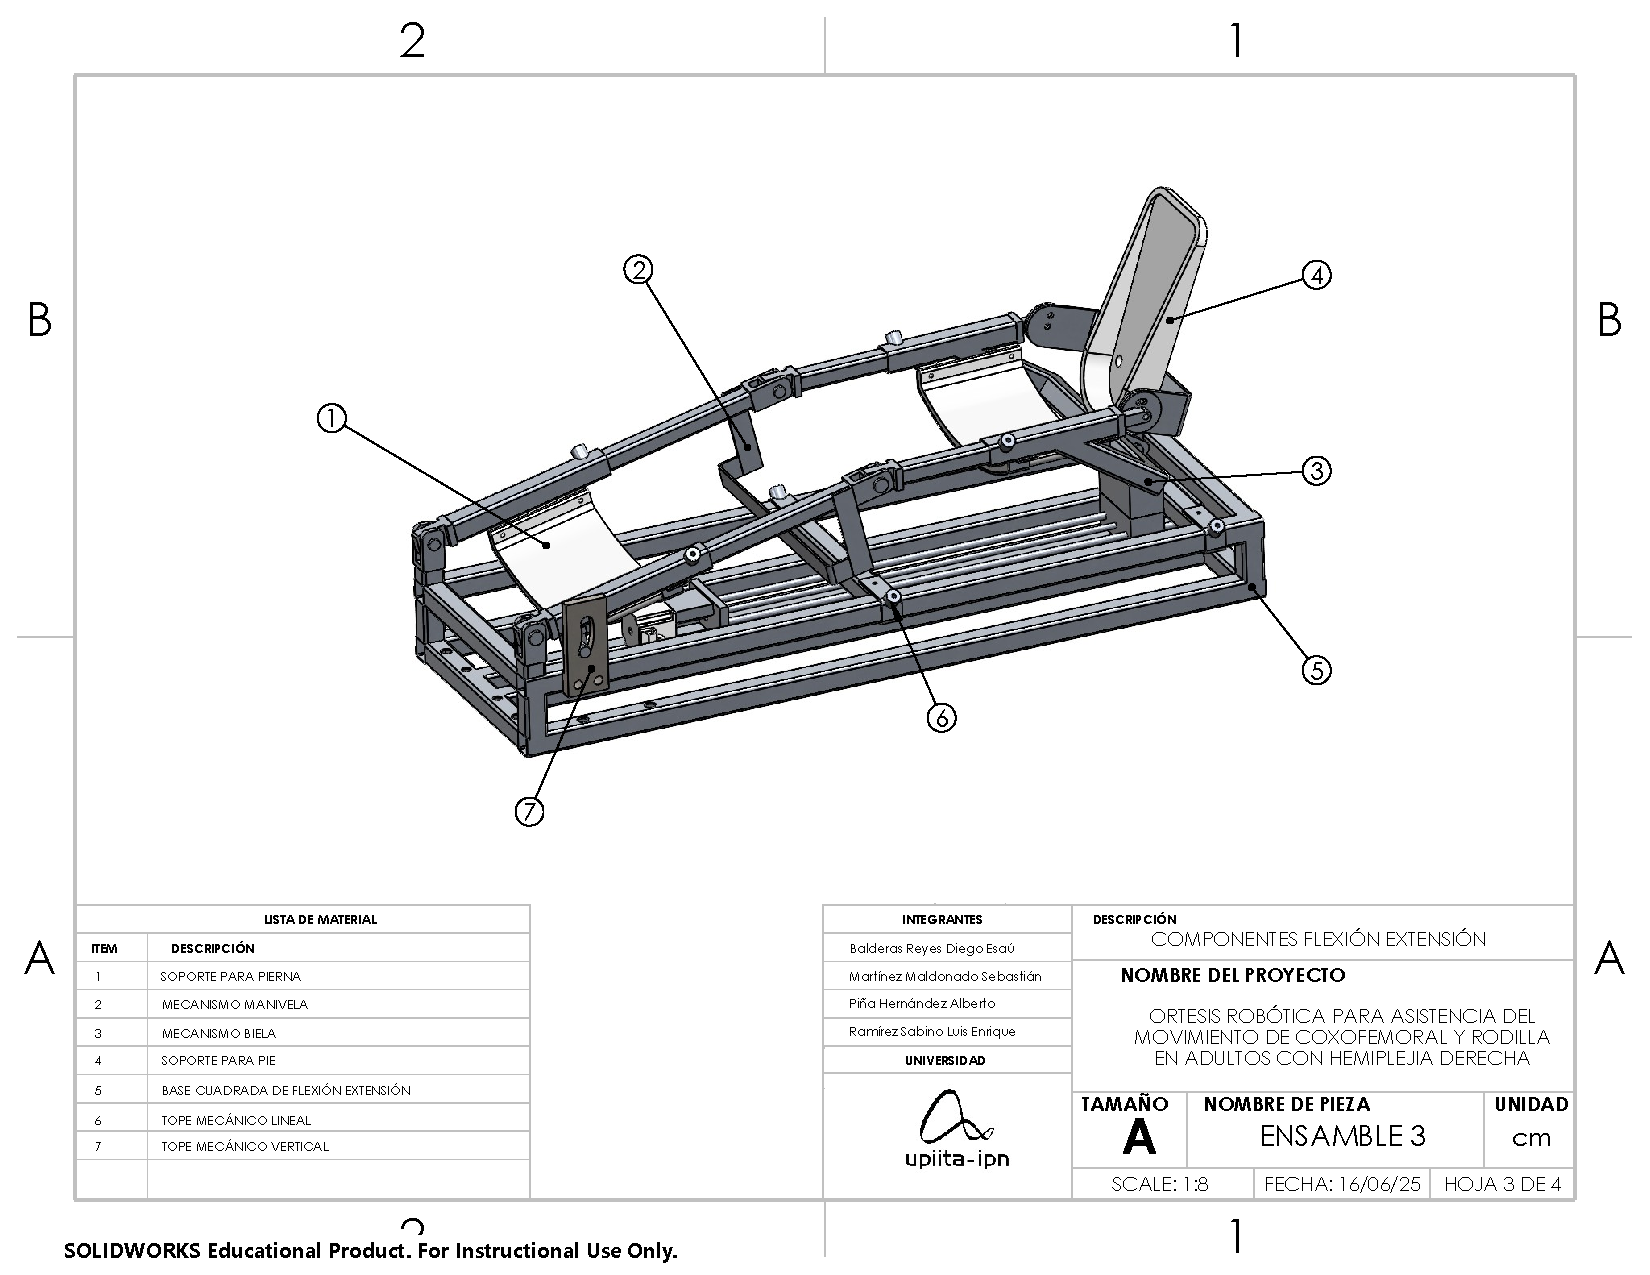
\includegraphics[trim={0 0cm 0 0},clip, angle =90, width=0.88\textwidth]{figure/planos_manufactura/Planos finales-3.pdf}
	\caption{Componentes flexión-extensión.}
	\label{fig:plano final 3}
	\end{figure}
    \begin{figure}[h!]
	\centering
	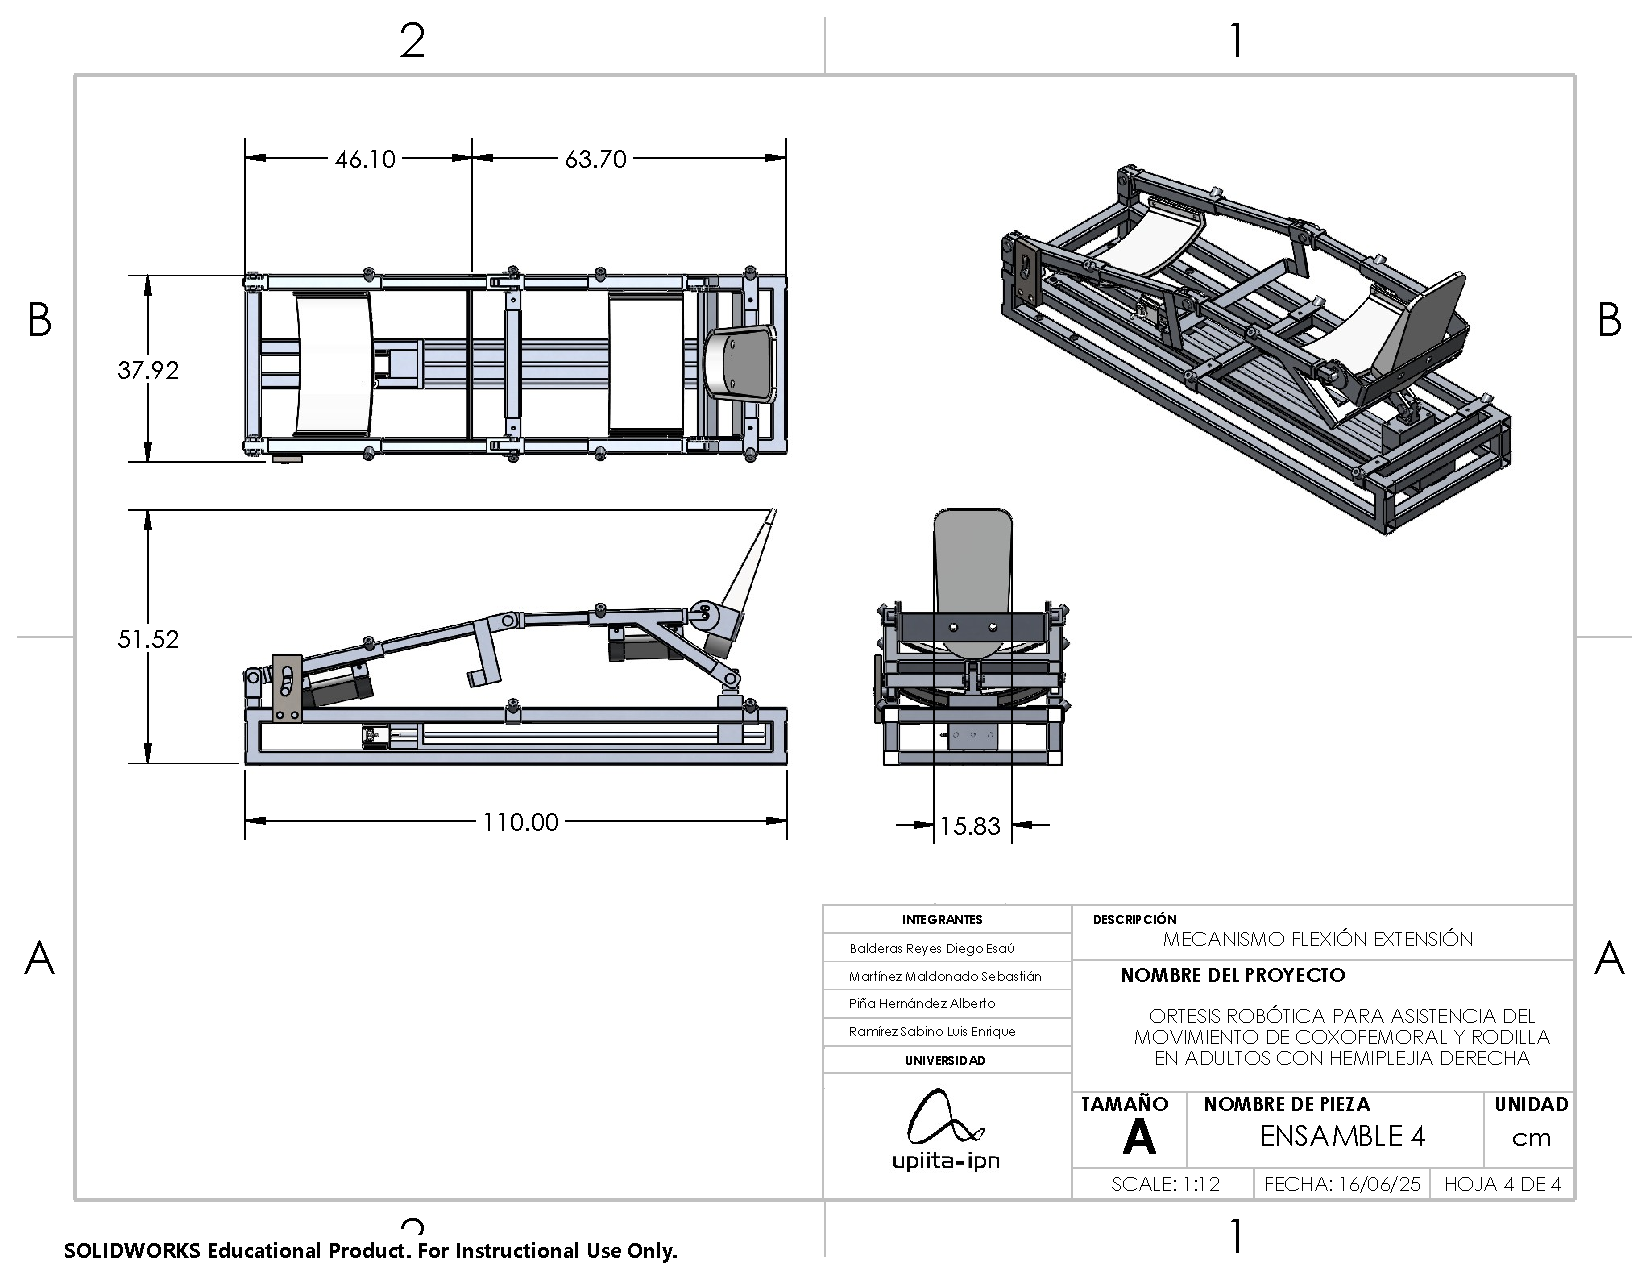
\includegraphics[trim={0 0cm 0 0},clip, angle =90, width=0.88\textwidth]{figure/planos_manufactura/Planos finales-4.pdf}
	\caption{Mecanismo de flexión-extensión.}
	\label{fig:plano final 4}
	\end{figure}
    
	 \section*{Apéndice B. Guía de mantenimiento y operación}\label{sec:planos de manufactura}
  \addcontentsline{toc}{section}{Apéndice B. Guía de mantenimiento y operación}
  Para garantizar la vida útil de los sistemas mecánicos y eléctricos, y asegurar la integridad del paciente, todas las labores de mantenimiento deben realizarse con el equipo desenergizado. Se debe seguir el siguiente plan periódico:
  \begin{itemize}
    \item \textbf{Chumaceras y rodamiento axial:} Requieren lubricación periódica con grasa industrial de litio cada 6 meses (o según la intensidad de uso), para asegurar que el motor Nema 34 transmita el par sin fricción excesiva durante la abducción-aducción.
    
    \item \textbf{Articulaciones (juntas Clevis):} Al ser uniones de fricción directa (aluminio 6061-T6 sin rodamientos internos), deben mantenerse libres de polvo y lubricadas con una capa ligera de lubricante seco para evitar la acumulación de partículas abrasivas. Se recomienda inspeccionar trimestralmente la aparición de holguras por desgaste.
    
    \item \textbf{Cableado y conexiones:} Realizar una inspección trimestral que incluya el reapriete de bornas en las fuentes conmutadas y drivers, así como la verificación del enclavamiento del contactor. Esto es crítico para prevenir falsos contactos derivados de las micro-vibraciones del sistema.
    
   \item \textbf{Limpieza de guías de deslizamiento:} Limpieza mensual de los rieles de aluminio del mecanismo de flexión-extensión utilizando un paño limpio y alcohol isopropílico. Es vital mantener la superficie libre de polvo para evitar el rayado del material y asegurar el desplazamiento suave del actuador lineal.

   \end{itemize}
	
%\end{appendices}